% !TEX root = main.tex

\section{Collecting and analyzing data}\label{sec:data}

Given the company context, a single tool approach was chosen as to not introduce extra dependencies/complexity (in contrast to combining different SA tools).\\
We use Clang AST \cite{clang_ast} and Clang Tidy \cite{clang_tidy} to analyze the code. We chose them because both are reliable and extensible open-source tools. Moreover, and most important, both are supported but the company's C++ codebase.


%\subsection{Collecting data}

\subsection{Clang AST}
Since some of the algorithms need metric data from the code, the Clang AST was chosen to extract that information. Assuming that the project can be successfully compiled, Clang can provide an API on top of the parsed AST.  

All information about the AST for a translation unit is bundled up in the class \textit{ASTContext}, which allows traversal of the whole translation unit.

Clang’s AST nodes are modeled on a class hierarchy that does not have a common ancestor and that consists of three main node types: Declarations, Statements (including Expressions) and Types (each with its own large inheritance hierarchy).

In order to traverse the AST, Clang offers two approaches:
\begin{itemize}
	\item \textbf{RecursiveASTVisitor}: A recursive visitor based approach, which allows you to run custom actions based on the node that is visited.
	\item \textbf{AST Matchers}: An approach that allows you to define what nodes you want to match by using a domain specific language.
\end{itemize}

\subsection{Clang Tidy}

Clang Tidy is a modular C++ linter tool which provides an extensible framework for diagnosing and fixing typical programming errors, like style violations, interface misuse, or bugs that can be deduced via static analysis \cite{clang_tidy}. 

In addition to its Static Analyzer checks, Clang Tidy contains a large list of other checks ranging from those that target bugprone code constructs, to CERT Secure Coding Guidelines, C++ Core Guidelines etc...

Clang Tidy can be configured by selecting the type of checks to be executed or by restricting the parts of code where to carry out such checks.

The following checks were regarded as relevant by the company and used during code analysis:
\begin{itemize}
	\item Clang Static Analyzer checks
	\item Checks related to C++ Core Guidelines
	\item Checks related to CERT Secure Coding Guidelines
	\item Checks related to performance
\end{itemize}

\subsection{Workflow for collecting data \label{data_collection}}

By exploiting the extensibility of Clang Tidy (ability to define new checks) and the power of the Clang AST (collecting information from code), the metrics needed by the ML algorithms can themselves be implemented as checks and thus be extracted automatically when analyzing the codebase. This is a flexible approach which allows to build automatic processing of alerts by integrating alert as well as metric collection within a single toolchain.

In order to make processing alerts easier, the C++ interface code of Clang Tidy was slightly changed to output information in a more suited format (line number instead of bit offset from start of file), hide not useful information, and output alerts only from the file under analysis (not from imported headers).

Starting by the provided open source \href{https://github.com/llvm-mirror/clang-tools-extra/blob/master/clang-tidy/tool/run-clang-tidy.py}{python scripts}, a workflow can be built in python to automatically collect alerts and metrics. In order to crawl the code history of the project, different script were implemented in python to automatically guide the workflow and process the output of SVN (version control system used at the company).

The high level workflow for collecting data consists of the following steps (see also \cref{data_workflow}):
\begin{itemize}
	\item Start by selecting a base revision in the code history.
	\item Fully analyze that revision of the codebase (collect all alerts output by Clang Tidy).
	\item Repeat for desired number of iterations (revisions):
	\begin{itemize}
		\item Checkout next revision, detect changed parts of code, collect surrounding information (author, changed methods, etc...).
		\item Run Clang Tidy only on the changed parts of code.
		\item Collect any new alerts and metrics.
	\end{itemize} 
\end{itemize}


\begin{figure}[H]
	\centering
	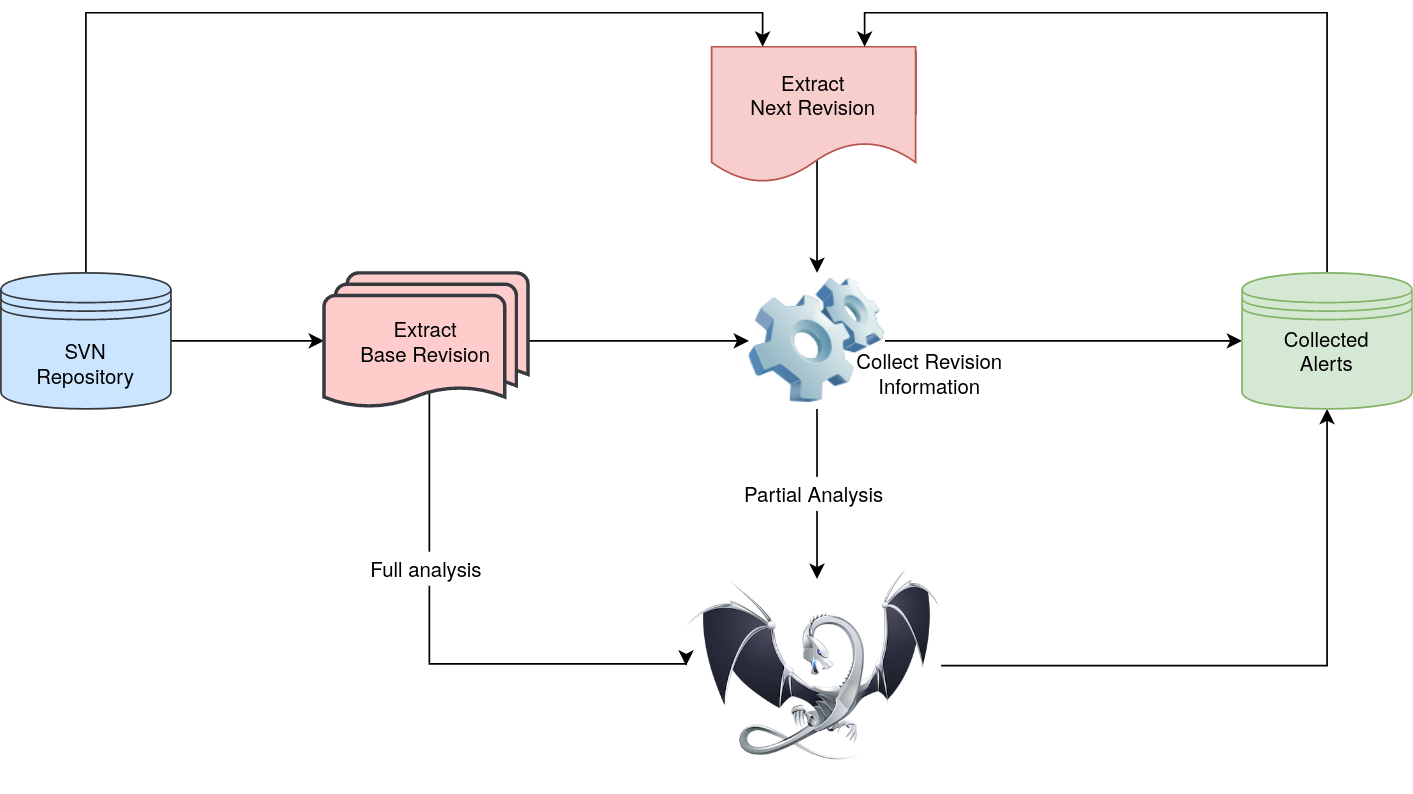
\includegraphics[scale=0.2]{./src/collect_info.png}
	\caption{Collecting alerts and other information}
	\label{data_workflow}
\end{figure}

\subsection{Assumptions made for collected data}
Some algorithms use the notion of \textit{Actionable Alerts} for processing the output of SA tools. Actionable Alerts (AA) are alerts that are deemed important by developers in the past (alerts that they acted on). In order to automatically label alerts as such (no existing information that can point to that), an important and risky assumption has to be made: alerts that disappear during code changes (revisions/commits) are considered as actionable, the rest is not. 

This assumptions, though necessary, is risky because not all alerts disappear as a result of direct and targeted change by developers. Their disappearance can be caused by other unknown factors (those related to deleted files are not taken into account). Data generated using this approach can contain a lot of false positives and potentially damage the performance of the used ML algorithms.

Another algorithm uses alerts pointing at past bugs as a way to prioritize future alerts. Also in this case an assumption is needed: the alerts that pointed to past bugs, were directly related to that bug. This may not always be true and can cause the aforementioned problems as a result.

The nature of automatic data extraction, without a reliable oracle pointing at the right decisions, leads to impure data and penalizes the efficiency of ML algorithms, but unfortunately it is an indispensable trade-off to be made.

\subsection{Data overview}

A typical release in the \textit{OMP's} codebase consists of around \textit{27.000} \textit{.cpp} files containing over \textit{4.000.000} lines and coded by more than 300 developers (in its entire history). The following section will provide a numerical overview of a portion of revisions analyzed from one of its releases 

We analyzed 1868 revisions, dating from \textit{09/2019} to \textit{05/2020}. From those revision, 1313 contain bug fixes. 

\subsubsection{Revision data}
We take a look at the main differences between normal and bug-fix commits.

%\henrique{When I said in Section 5 that tables need to have a number and a title/caption, I meant it for the entire thesis. The tables bellow are missing that.}
%\kleidi{Did not want to change all sections and cause possible merge conflicts on your part...}

\begin{table}[H]
	\centering
	\caption{File/Method change metrics in collected revision}
	\label{rev_files}
	\begin{tabular}{@{}lcccc@{}}
		\toprule
		& \multicolumn{1}{l}{\textbf{Modified Files}} & \multicolumn{1}{l}{\textbf{Added Files}} & \multicolumn{1}{l}{\textbf{Deleted Files}} & \multicolumn{1}{l}{\textbf{Modified Methods}} \\ \midrule
		& \multicolumn{4}{c}{\textbf{MEAN}}                                                                                                                                                   \\
		\textit{Normal}  & 7                                           & 1.4                                      & 0.98                                       & 6.8                                           \\
		\textit{Bug-Fix} & 4.3                                         & 0.52                                     & 0.21                                       & 4.64                                          \\
		& \multicolumn{1}{l}{}                        & \multicolumn{1}{l}{}                     & \multicolumn{1}{l}{}                       & \multicolumn{1}{l}{}                          \\
		& \multicolumn{4}{c}{\textbf{MEDIAN}}                                                                                                                                                 \\
		\textit{Normal}  & 2                                           & 0                                        & 0                                          & 1                                             \\
		\textit{Bug-Fix} & 3                                           & 0                                        & 0                                          & 2                                             \\ \bottomrule
	\end{tabular}
\end{table}

\begin{table}[H]
	\centering
	\caption{Line change metrics in collected revision}
	\label{rev_lines}
	\begin{tabular}{@{}lcccc@{}}
		\toprule
		& \multicolumn{1}{l}{\textbf{Added Lines}} & \multicolumn{1}{l}{\textbf{Deleted Lines}} & \multicolumn{1}{l}{\textbf{Modified Lines}} & \multicolumn{1}{l}{\textbf{Growth Lines}} \\ \midrule
		& \multicolumn{4}{c}{\textbf{MEAN}}                                                                                                                                               \\
		\textit{Normal}  & 99.8                                     & 40.2                                       & 140                                         & 59.7                                      \\
		\textit{Bug-Fix} & 47.8                                     & 24.5                                       & 72.3                                        & 23.3                                      \\
		& \multicolumn{1}{l}{}                     & \multicolumn{1}{l}{}                       & \multicolumn{1}{l}{}                        & \multicolumn{1}{l}{}                      \\
		& \multicolumn{4}{c}{\textbf{MEDIAN}}                                                                                                                                             \\
		\textit{Normal}  & 16                                       & 6                                          & 26                                          & 2                                         \\
		\textit{Bug-Fix} & 9                                        & 4                                          & 14                                          & 2                                         \\ \bottomrule
	\end{tabular}
\end{table}

 \begin{figure}[H]
	\begin{subfigure}{.5\textwidth}
		\centering
		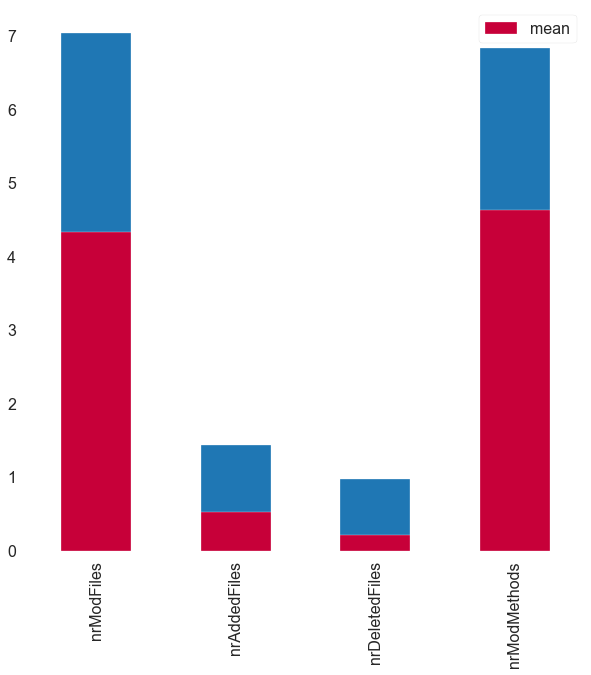
\includegraphics[scale=0.3]{./src/data_analysis/rev_files.png}
	\end{subfigure}%
	\begin{subfigure}{.5\textwidth}
		\centering
		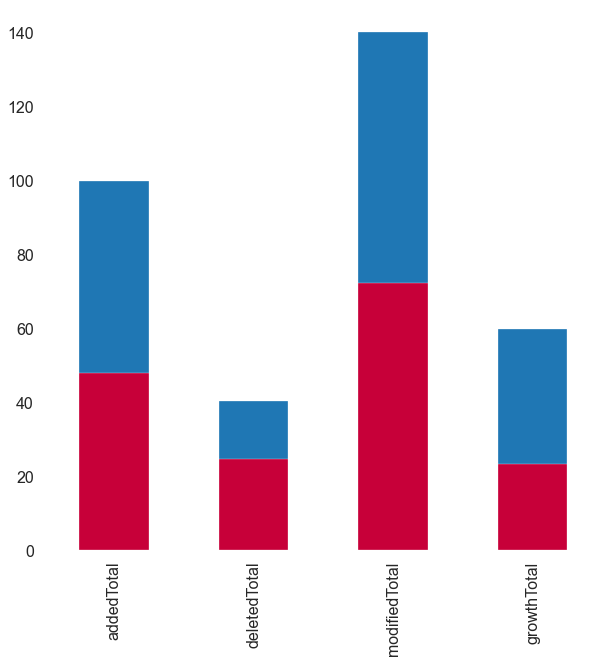
\includegraphics[scale=0.3]{./src/data_analysis/rev_lines.png}
	\end{subfigure}
	\caption{Average changes (\textit{red=bug revision, blue=normal})}
	\label{rev_changes}
\end{figure}

As can be seen from the data (\cref{rev_files}, \cref{rev_lines}, and \cref{rev_changes}), there is significant difference between the amount of changes that happen during a normal and a bug-fix revision, with the later being almost half the size. That is important because the bug fix changes can be better located. There is also a big difference between mean and median values of the collected features, shifting the values of the former to be higher (can be also seen on the box plots on \cref{box:changed_lines} and \cref{box:changed_files}). That means that there are certain revision that are abnormally large compared to others and that negatively impact the quality of the data. 

\begin{figure}[H]
	\begin{subfigure}{0.5\textwidth}
		\centering
		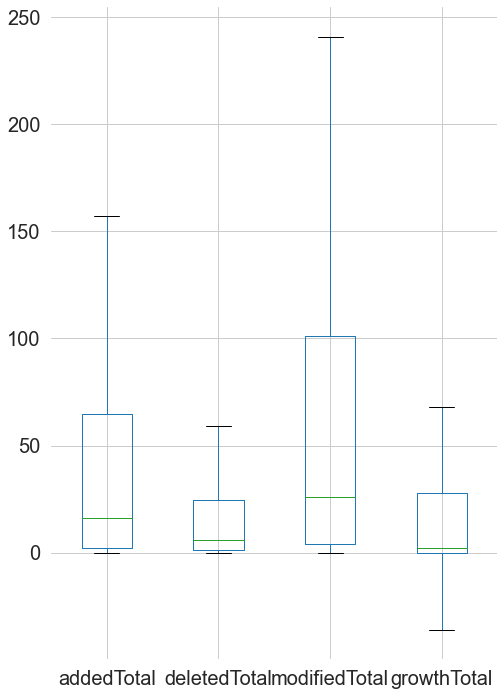
\includegraphics[scale=0.3]{./src/data_analysis/normal_box_lines.png}
		\caption{Box plots for changed lines in normal revisions}
	\end{subfigure}%
	\begin{subfigure}{0.5\textwidth}
		\centering
		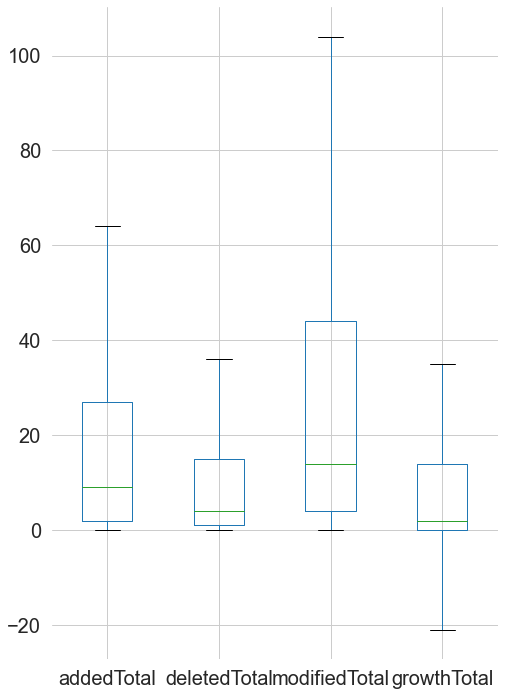
\includegraphics[scale=0.3]{./src/data_analysis/buggy_box_lines.png}
		\caption{Box plots for changed lines in buggy revisions}
	\end{subfigure}
	\caption{}
	\label{box:changed_lines}
\end{figure}

\begin{figure}[H]
	\begin{subfigure}{0.5\textwidth}
		\centering
		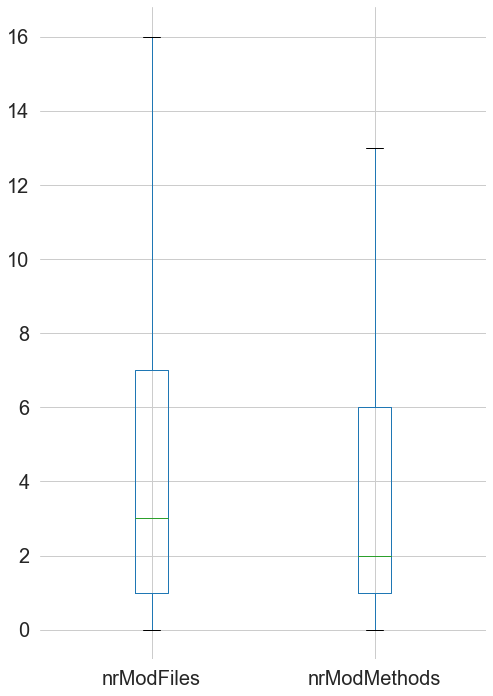
\includegraphics[scale=0.3]{./src/data_analysis/normal_box_files.png}
		\caption{Box plots for changed files/methods in normal revisions}
	\end{subfigure}%
	\begin{subfigure}{0.5\textwidth}
		\centering
		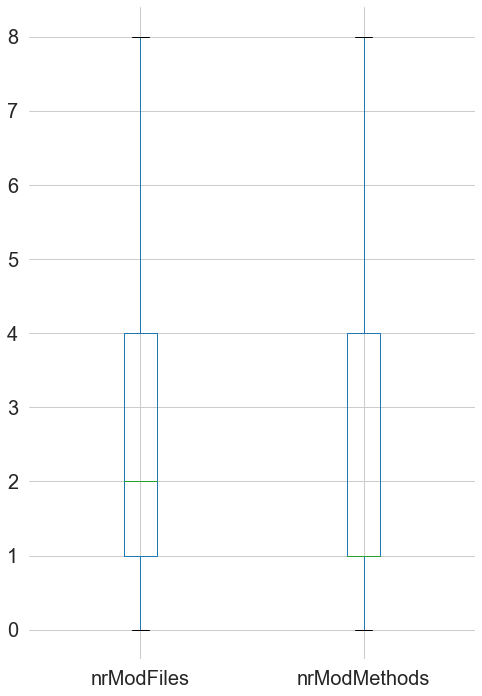
\includegraphics[scale=0.3]{./src/data_analysis/buggy_box_files.png}
		\caption{Box plots for changed files/methods in buggy revisions}
	\end{subfigure}
	\caption{}
	\label{box:changed_files}
\end{figure}

\newpage
\subsubsection{Closed Alerts}

\begin{table}[H]
	\centering
	\begin{tabular}{@{}lcccc@{}}
		\toprule
		& \textbf{Number of alert} & \textbf{\% of alerts} & \textbf{Number of closed alerts} & \textbf{\% of closed alerts} \\ \midrule
		\textit{cppcoreguidelines} & 177812                   & 93.8\%                & 78785                            & 95.6\%                       \\
		\textit{performance}       & 6010                     & 3.2\%                 & 2297                             & 2.8\%                        \\
		cert                       & 4673                     & 2.5\%                 & 948                              & 1.2\%                        \\
		\textit{clang}             & 1040                     & 0.5\%                 & 346                              & 0.4\%                        \\ \bottomrule
	\end{tabular}
\end{table}
\begin{figure}[H]
	\centering
	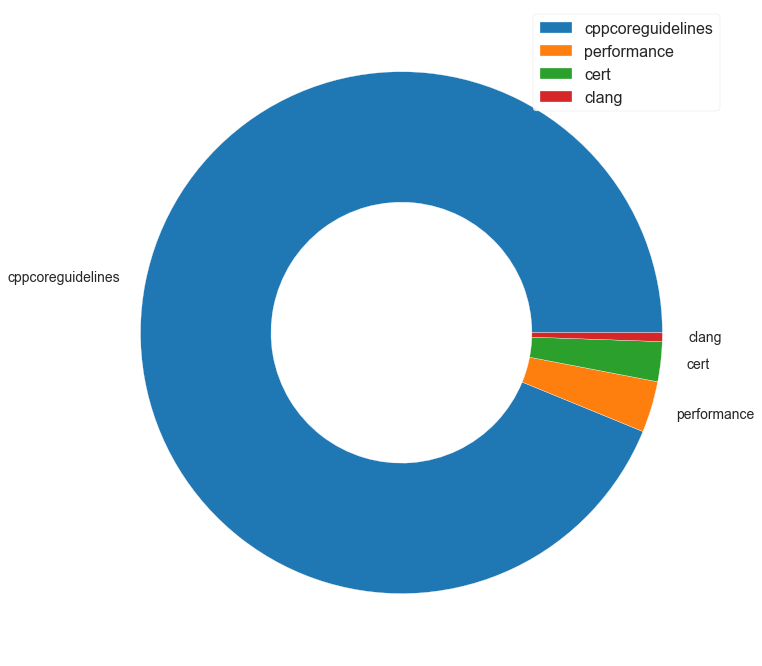
\includegraphics[scale=0.4]{./src/data_analysis/pie_alerts.png}
	\caption{Distribution of collected alerts per alert category}
\end{figure}

From the distribution of collected alerts, we can see that it is dominated by the \textit{cppcoreguidelines} checks, while the remaining three categories consist only of 4.4\% of the total alerts.

\begin{table}[H]
	\centering
	\begin{tabular}{lcc}
		\hline
		& \textbf{Number of closed alerts} & \textbf{\% of closed alerts inside category} \\ \hline
		\textit{cppcoreguidelines} & 78785                            & 44\%                                         \\
		\textit{performance}       & 2297                             & 38\%                                         \\
		cert                       & 948                              & 20\%                                         \\
		\textit{clang}             & 346                              & 33\%                                         \\ \hline
	\end{tabular}
\end{table}

\begin{figure}[H]
	\centering
	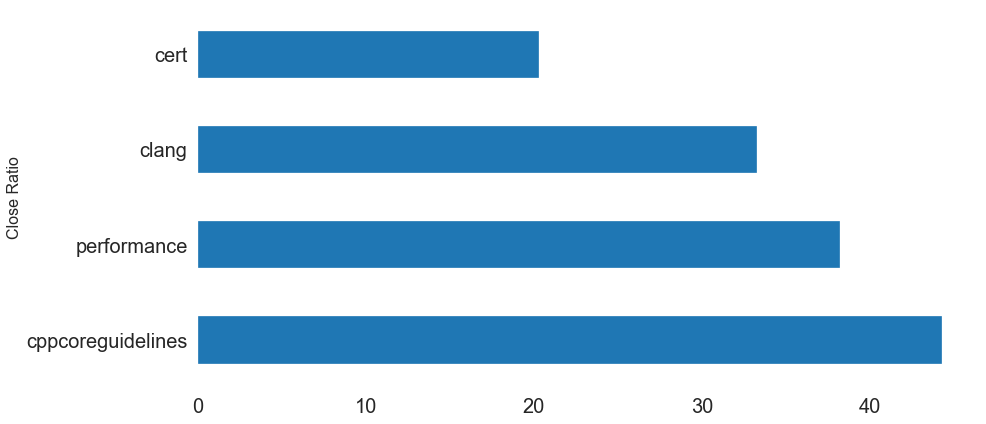
\includegraphics[scale=0.4]{./src/data_analysis/closed_ratio_category.png}
	\caption{Ratio of closed alerts per category}
\end{figure}

The ratio of closed alerts inside each category also differs greatly, from 44\% of \textit{cppcoreguidelines} to 20\% of the \textit{cert} alerts.

By analyzing the lifetime of closed alerts, in terms of number of revisions, we can see that alerts take before getting closed (see \cref{closed_alerts:lifetime}). Around a quart of alerts gets closed within 200 first revisions after being opened. That is not a good indication because it may mean that they do not directly disappear from targeted action from developers.

\begin{figure}[h]
	\begin{subfigure}{1\textwidth}
		\centering
		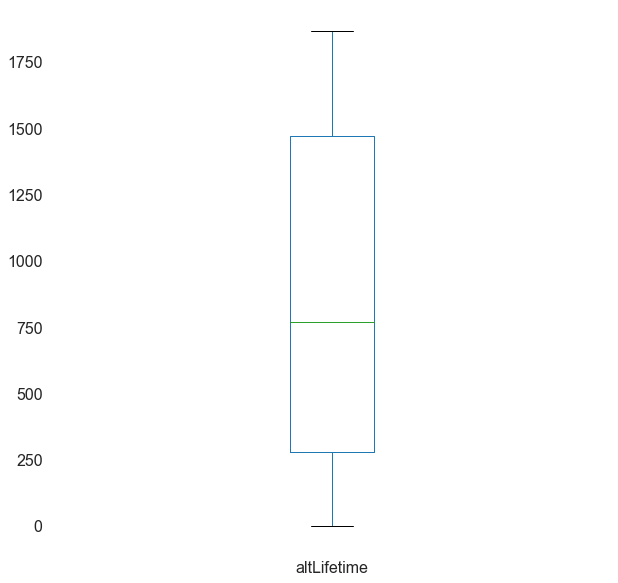
\includegraphics[scale=0.3]{./src/data_analysis/alert_lifetime_box.png}
		\caption{Box plot for closed alert lifetime}
	\end{subfigure}\\
	\begin{subfigure}{1\textwidth}
		\begin{subfigure}{.5\textwidth}
			\centering
			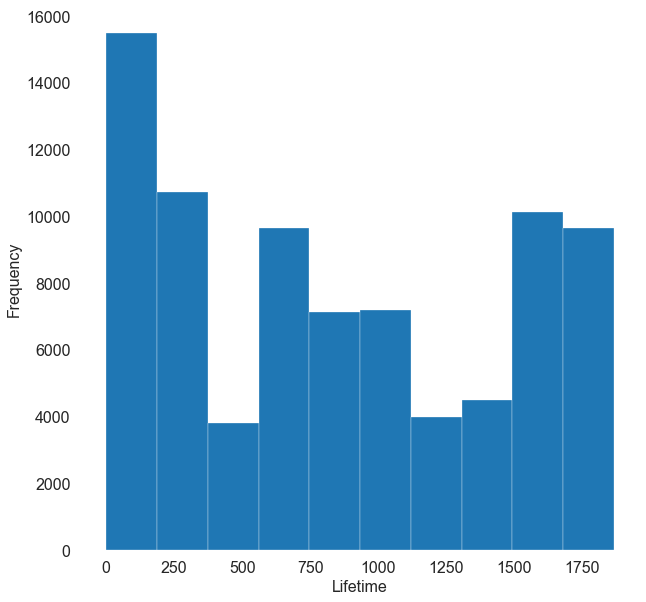
\includegraphics[scale=0.3]{./src/data_analysis/alert_lifetime_hist.png}
			\caption{Histogram for closed alert lifetime}
		\end{subfigure}%
		\begin{subfigure}{.5\textwidth}
			\centering
			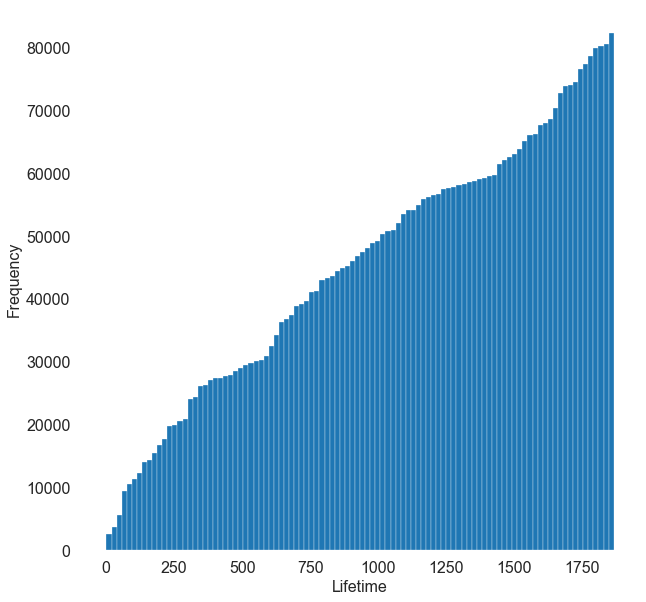
\includegraphics[scale=0.3]{./src/data_analysis/alert_lifetime_cumulative.png}
			\caption{Cumulative plot for closed alert lifetime}
		\end{subfigure}
	\end{subfigure}
	\caption{}
	\label{closed_alerts:lifetime}
\end{figure}


\begin{figure}[H]
	\begin{subfigure}{0.5\textwidth}
		\centering
		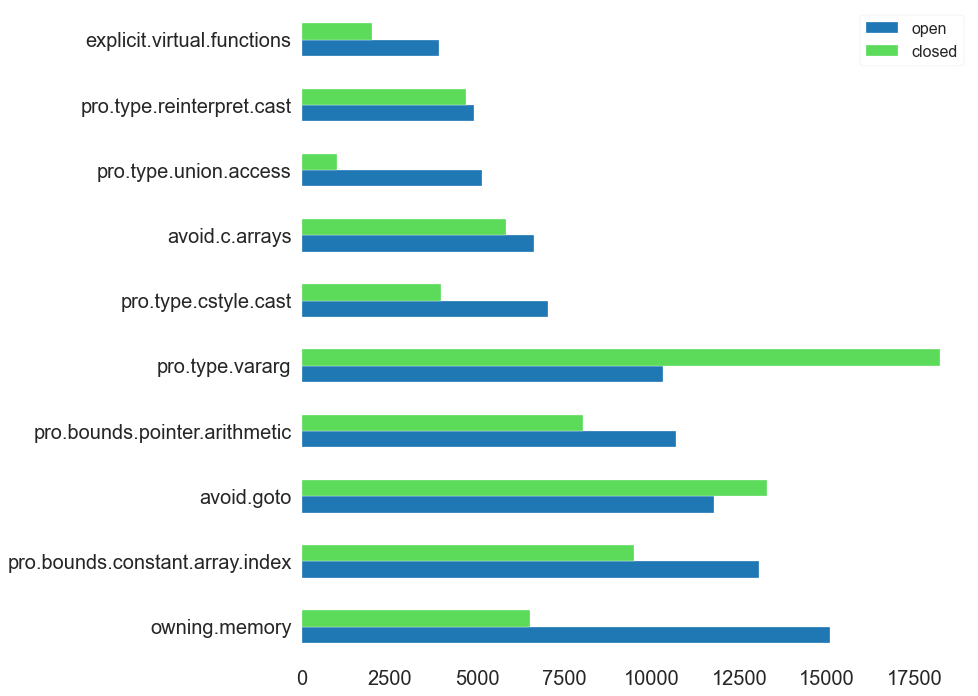
\includegraphics[scale=0.2]{./src/data_analysis/most_open_alerts.png}
		\caption{Bar plot for alert types with most open alerts}
	\end{subfigure}%
	\begin{subfigure}{0.5\textwidth}
		\centering
		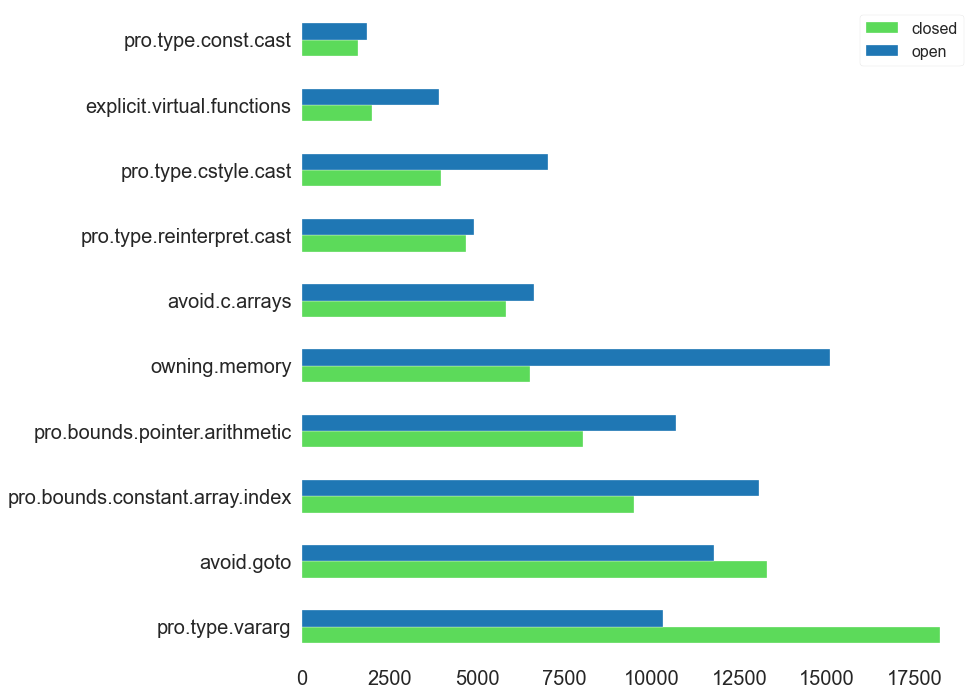
\includegraphics[scale=0.2]{./src/data_analysis/most_closed_alerts.png}
		\caption{Bar plot for alert types with most closed alerts}
	\end{subfigure}
	\caption{}
	\label{most_open_alerts}
\end{figure}


\begin{figure}[H]
	\begin{subfigure}{0.5\textwidth}
		\centering
		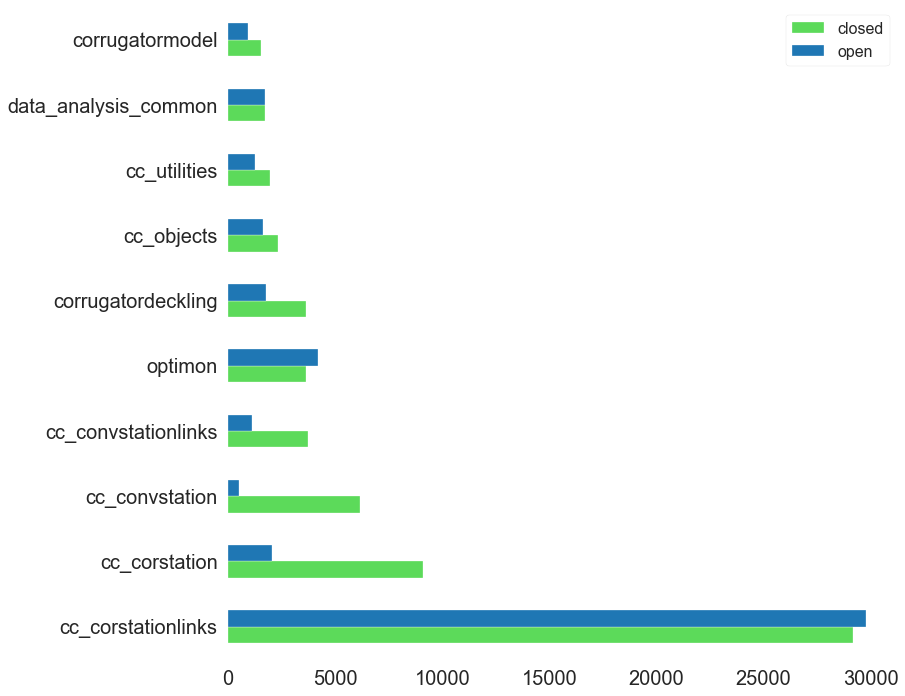
\includegraphics[scale=0.2]{./src/data_analysis/most_open_packages.png}
		\caption{Bar plot for packages with most open alerts}
	\end{subfigure}%
	\begin{subfigure}{0.5\textwidth}
		\centering
		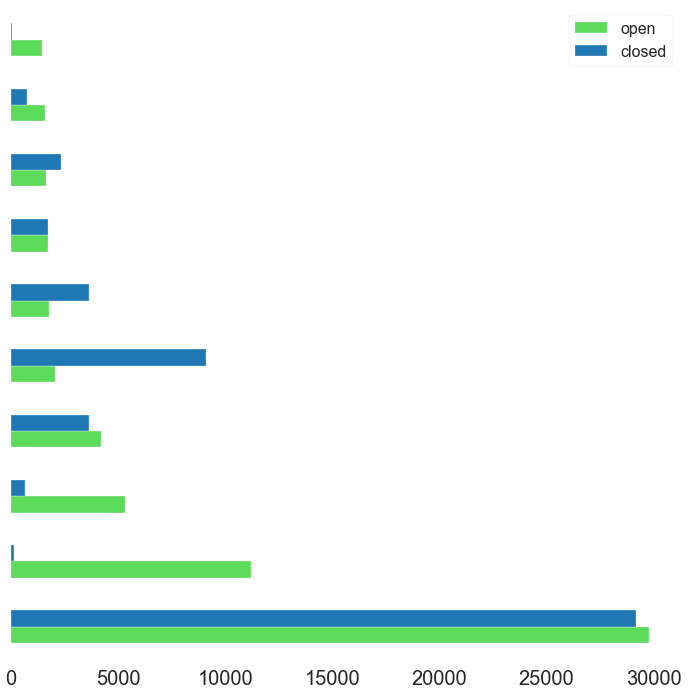
\includegraphics[scale=0.2]{./src/data_analysis/most_closed_packages.png}
		\caption{Bar plot for packages with most closed alerts}
	\end{subfigure}
	\caption{}
	\label{most_open_packages}
\end{figure}

From the plots in \cref{most_open_alerts} and \cref{most_open_packages}, we can see that the distribution of open/closed alerts is dominated on an package level. The package \textit{cc\_corstationlinks} contains half of the closed alerts. There exists thus a heavy imbalance in terms of the location of closed alerts.


%\begin{figure}[H]
%	\begin{subfigure}{\textwidth}
%		\centering
%		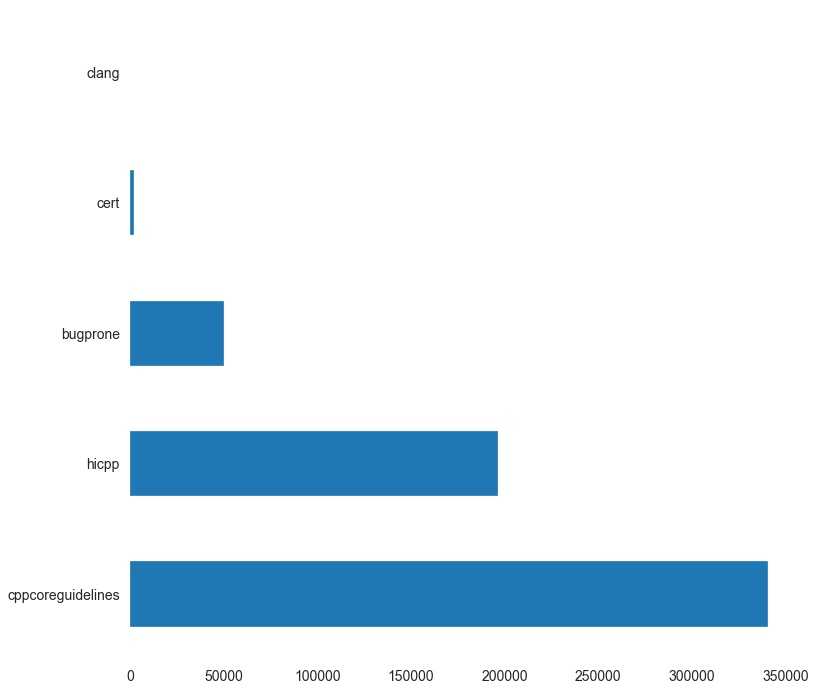
\includegraphics[scale=0.3]{./src/data_analysis/category_barh.jpg}
%		\caption{Alert categories for collected alerts}\label{}
%	\end{subfigure}\\
%	\begin{subfigure}{.5\textwidth}
%		\centering
%		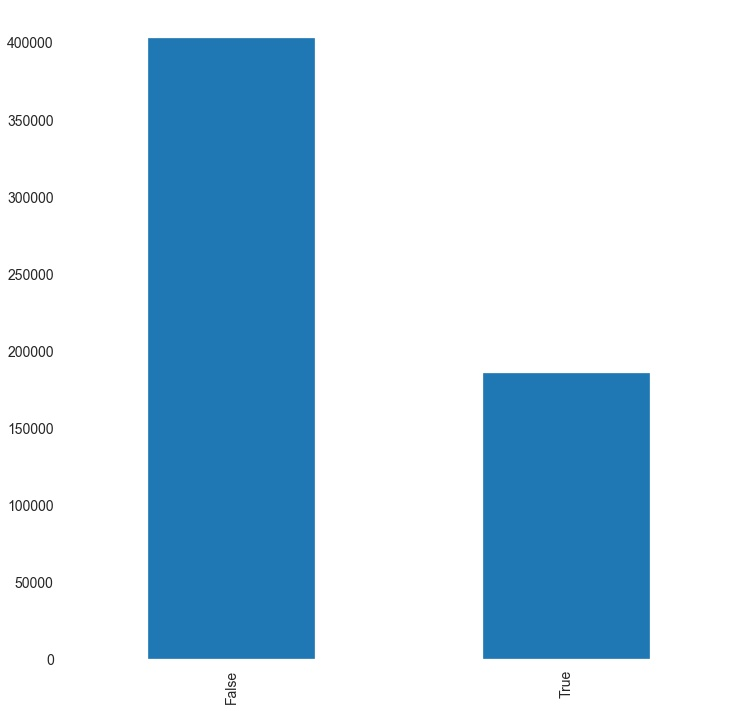
\includegraphics[scale=0.3]{./src/data_analysis/open_close_alerts.jpg}
%		\caption{Number of open and closed alerts}\label{}
%	\end{subfigure}%
%	\begin{subfigure}{.5\textwidth}
%		\centering
%		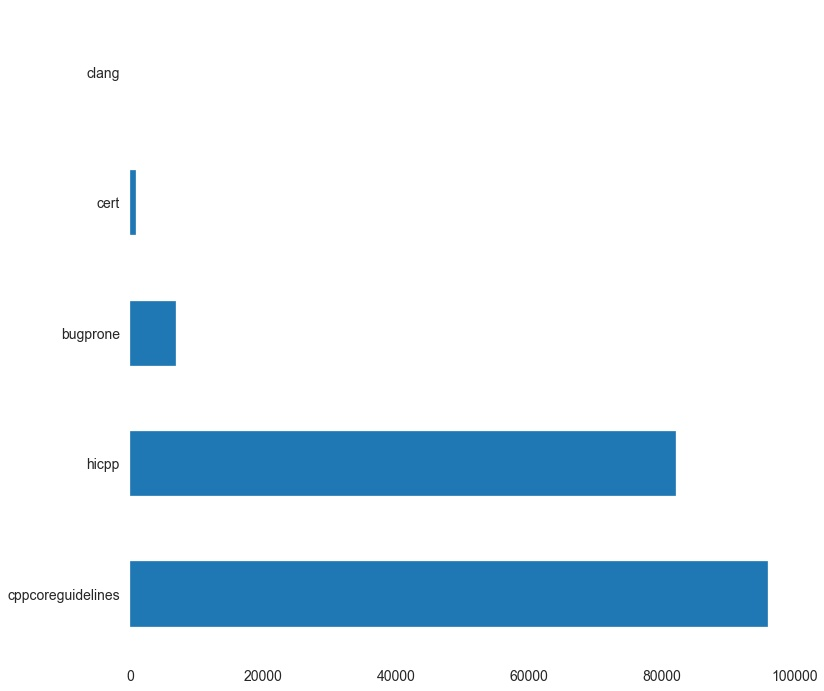
\includegraphics[scale=0.3]{./src/data_analysis/closed_category_barh.jpg}
%		\caption{Number of closed alerts per category}\label{}
%	\end{subfigure}  
%\end{figure}
%
%As can be seen from the plots, there is a mismatch between the number of open/closed alerts, as well as alerts categories (some of them are under represented like clang/cert).
%
%
%\begin{figure}[H]
%	\begin{subfigure}{0.5\textwidth}
%		\centering
%		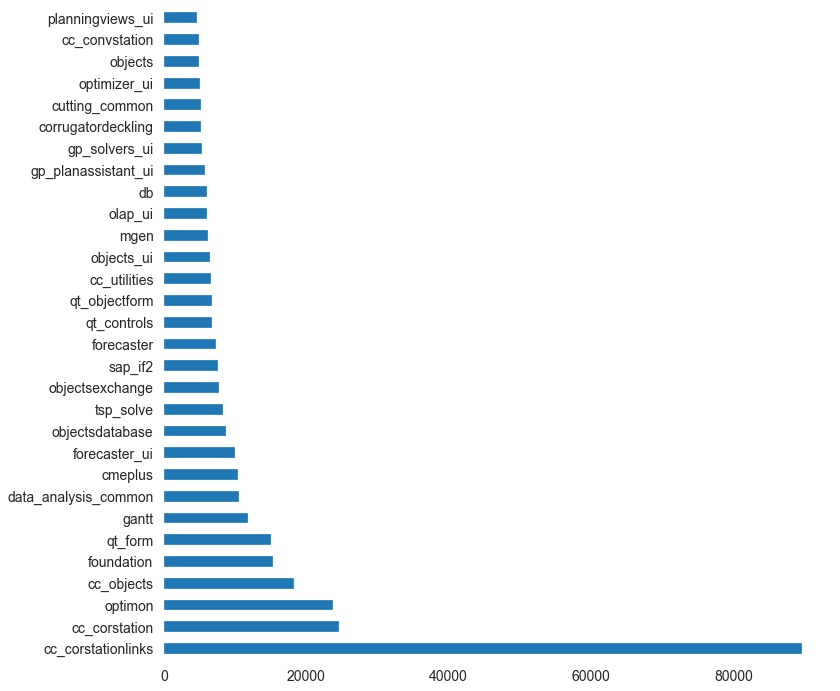
\includegraphics[scale=0.3]{./src/data_analysis/alerts_packages_barh.jpg}
%		\caption{Number of alerts in the 30 most represented packages}\label{}
%	\end{subfigure}%
%	\begin{subfigure}{0.5\textwidth}
%		\centering
%		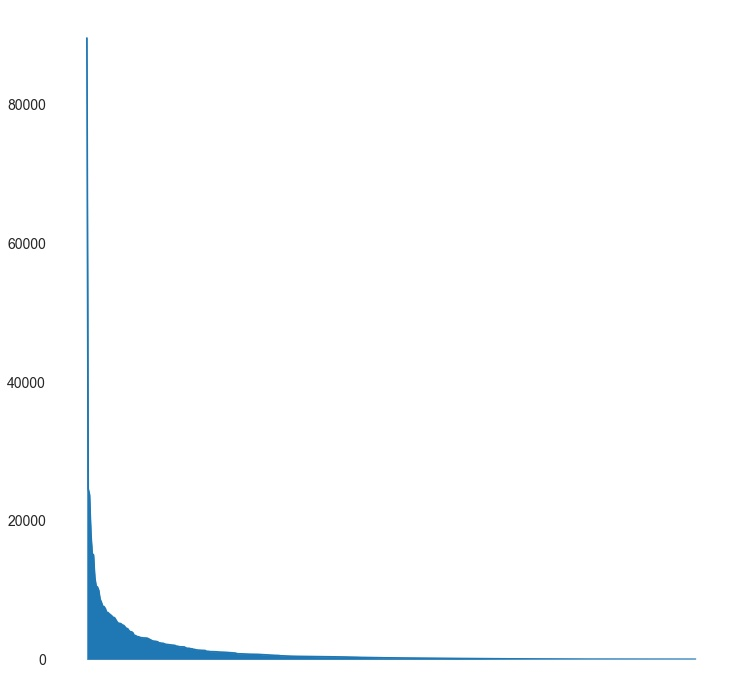
\includegraphics[scale=0.3]{./src/data_analysis/alerts_packages_area.jpg}
%		\caption{Plot of number of alerts per package}\label{}
%	\end{subfigure}\\
%	\begin{subfigure}{\textwidth}
%		\centering
%		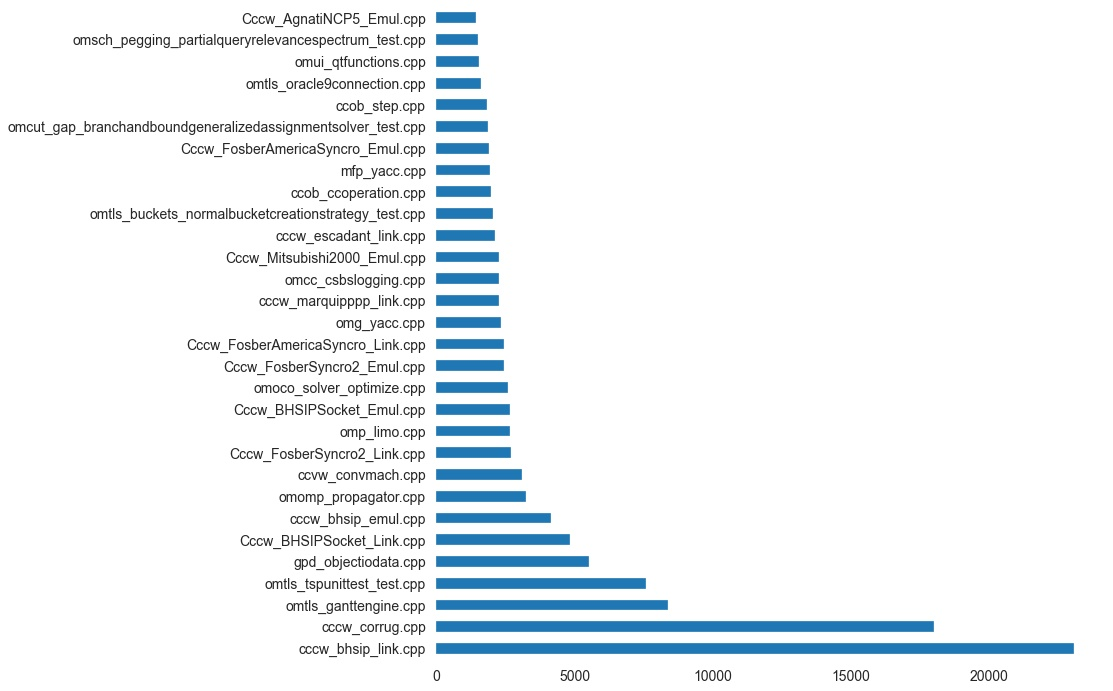
\includegraphics[scale=0.3]{./src/data_analysis/alerts_files_barh.jpg}
%		\caption{Number of alerts in the 30 most represented files}\label{}
%	\end{subfigure}%
%	%	\begin{subfigure}{0.5\textwidth}
%	%		\centering
%	%		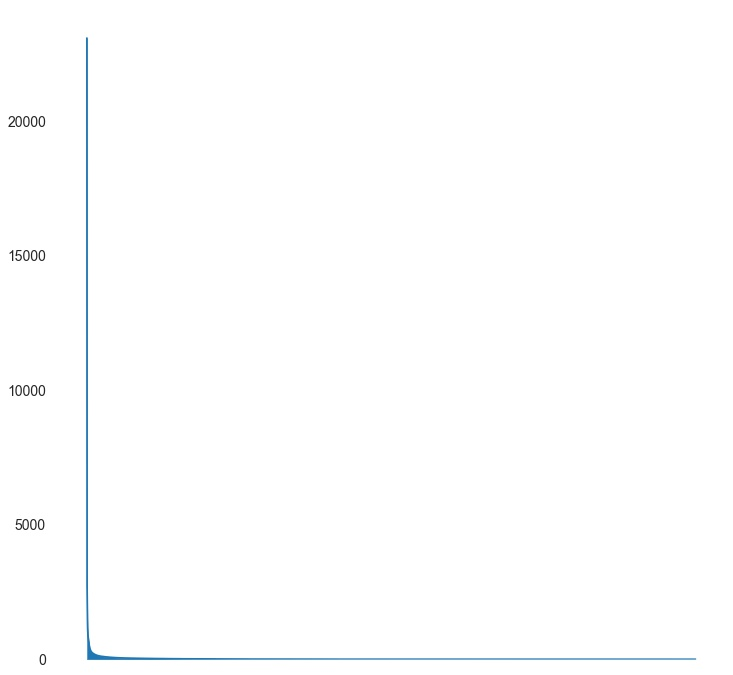
\includegraphics[scale=0.2]{./src/data_analysis/alerts_files_area.jpg}
%	%		\caption{Plot of number of alerts per file}\label{}
%	%	\end{subfigure}  
%\end{figure}
%
%Regarding the distribution of the alerts in packages and files, we see similar trends: some of the packages/files contain a big chunk of the total alerts and most of them contain little to no alerts. 
%
%\begin{figure}[H]
%	\begin{subfigure}{0.5\textwidth}
%		\centering
%		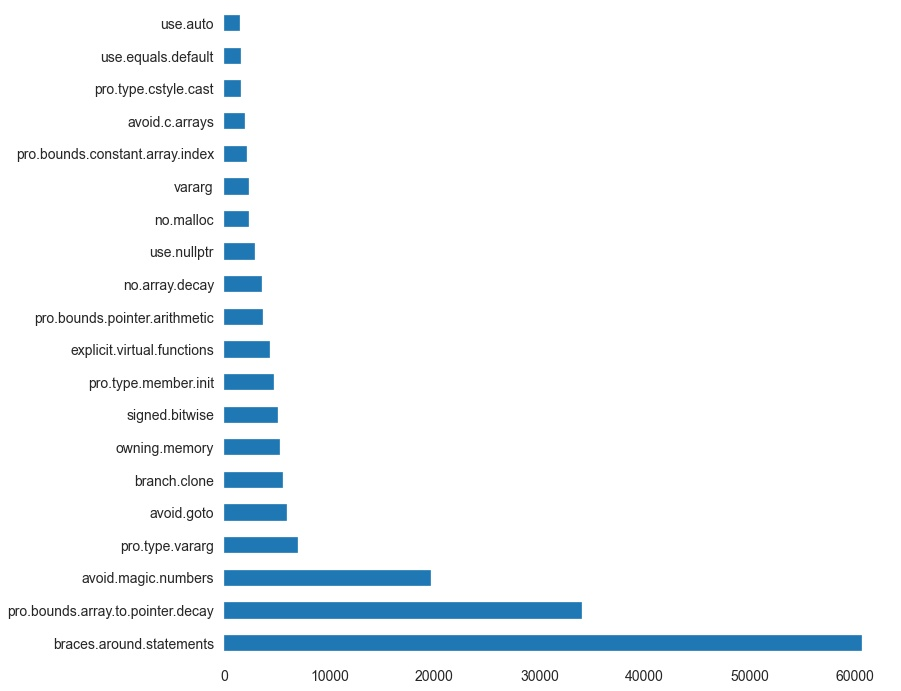
\includegraphics[scale=0.2]{./src/data_analysis/closed_types_barh.jpg}
%		\caption{Number of open alerts in the 30 most represented types}\label{}
%	\end{subfigure}%
%	\begin{subfigure}{0.5\textwidth}
%		\centering
%		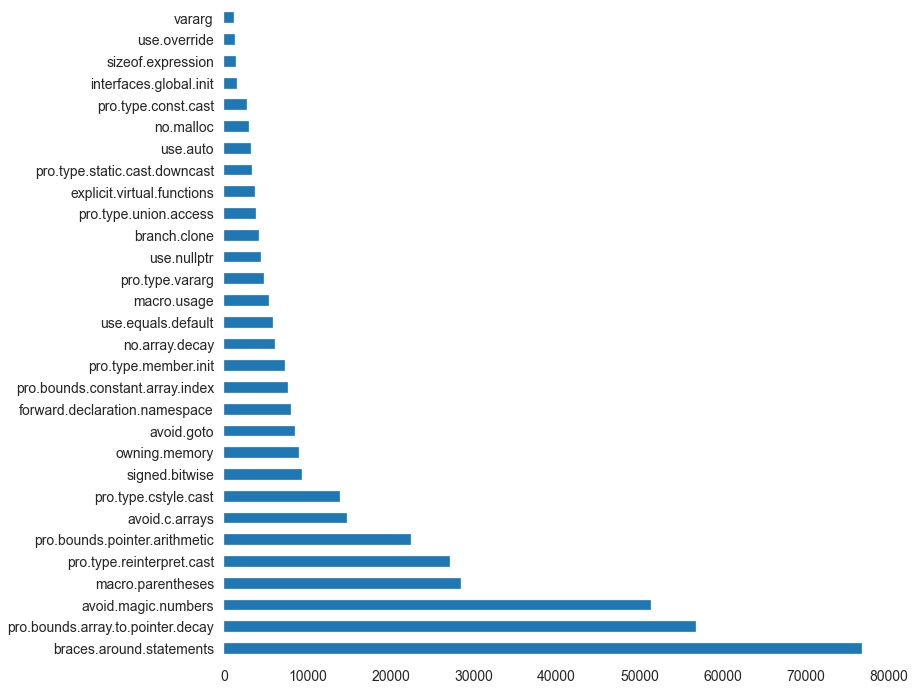
\includegraphics[scale=0.2]{./src/data_analysis/open_type_barh.jpg}
%		\caption{Number of closed alerts in the 30 most represented types}\label{}
%	\end{subfigure}
%	\begin{subfigure}{0.5\textwidth}
%		\centering
%		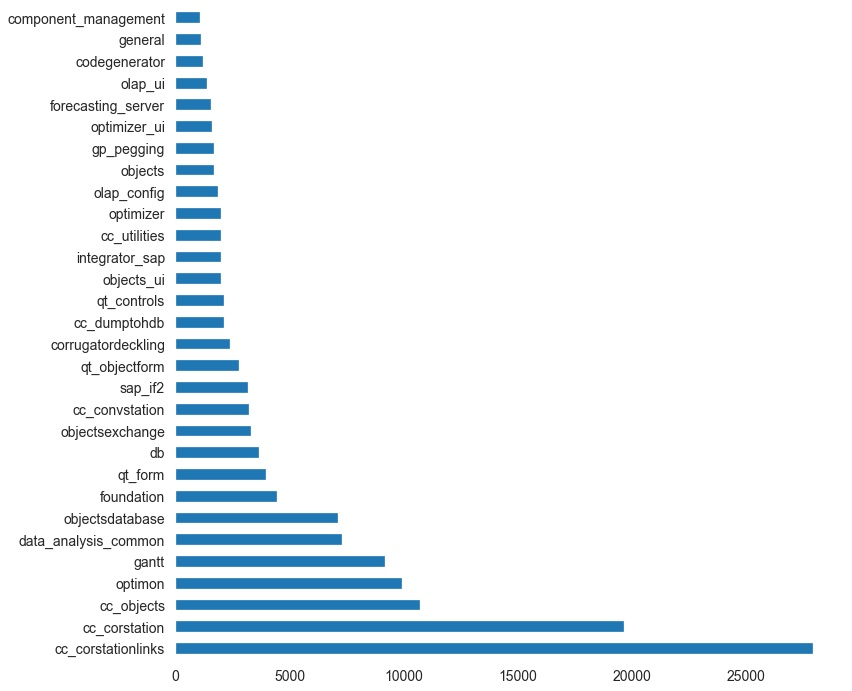
\includegraphics[scale=0.2]{./src/data_analysis/closed_packages_barh.jpg}
%		\caption{Number of open alerts in the 30 most represented packages}\label{}
%	\end{subfigure}%
%	\begin{subfigure}{0.5\textwidth}
%		\centering
%		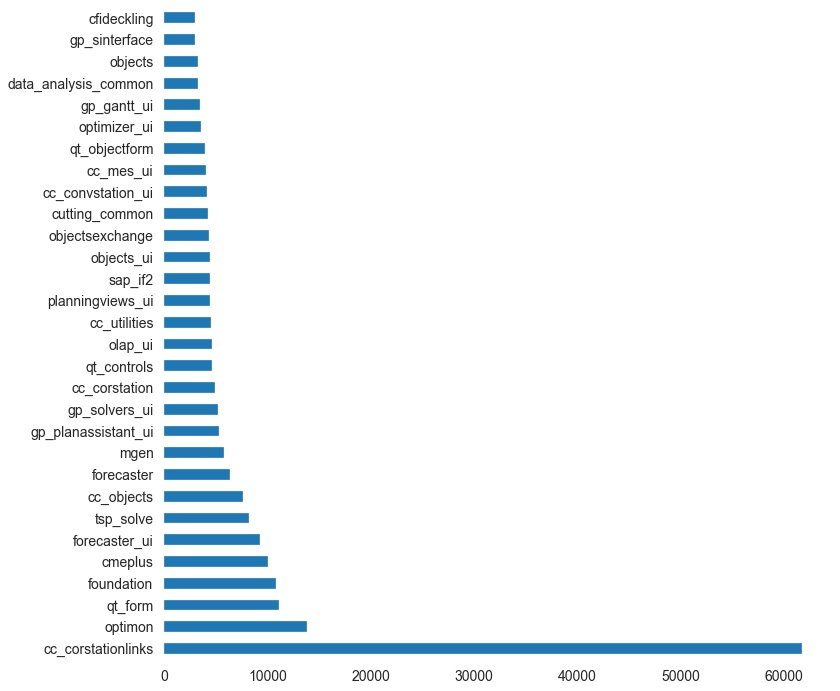
\includegraphics[scale=0.2]{./src/data_analysis/open_package_barh.jpg}
%		\caption{Number of closed alerts in the 30 most represented packages}\label{}
%	\end{subfigure}\\
%	\begin{subfigure}{0.5\textwidth}
%		\centering
%		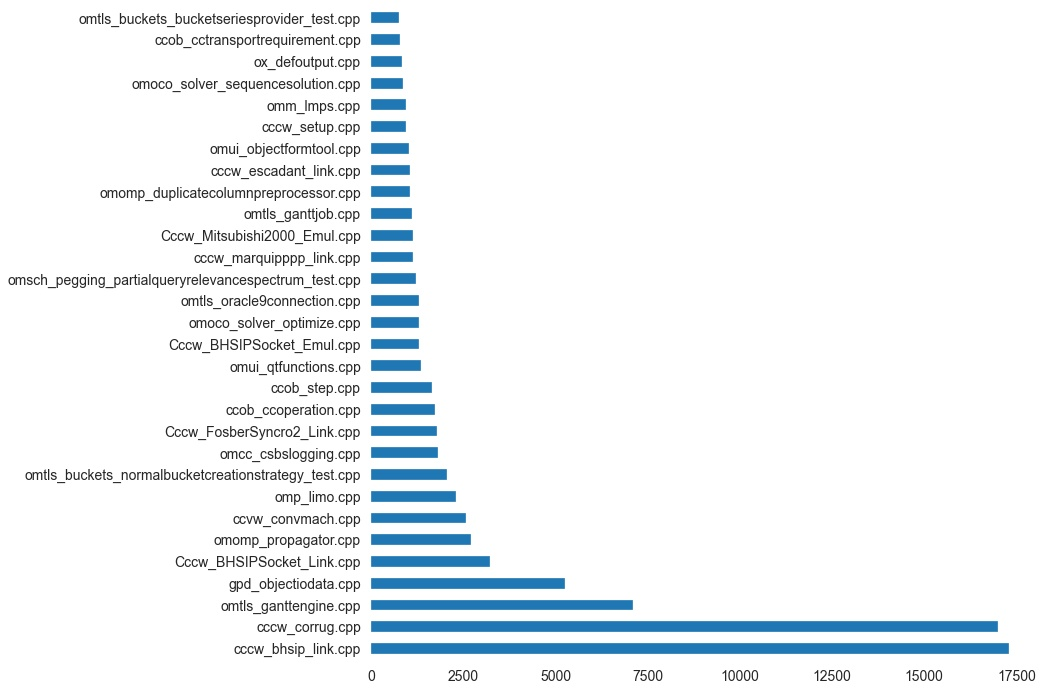
\includegraphics[scale=0.2]{./src/data_analysis/closed_files_barh.jpg}
%		\caption{Number of open alerts in the 30 most represented files}\label{}
%	\end{subfigure}%
%	\begin{subfigure}{0.5\textwidth}
%		\centering
%		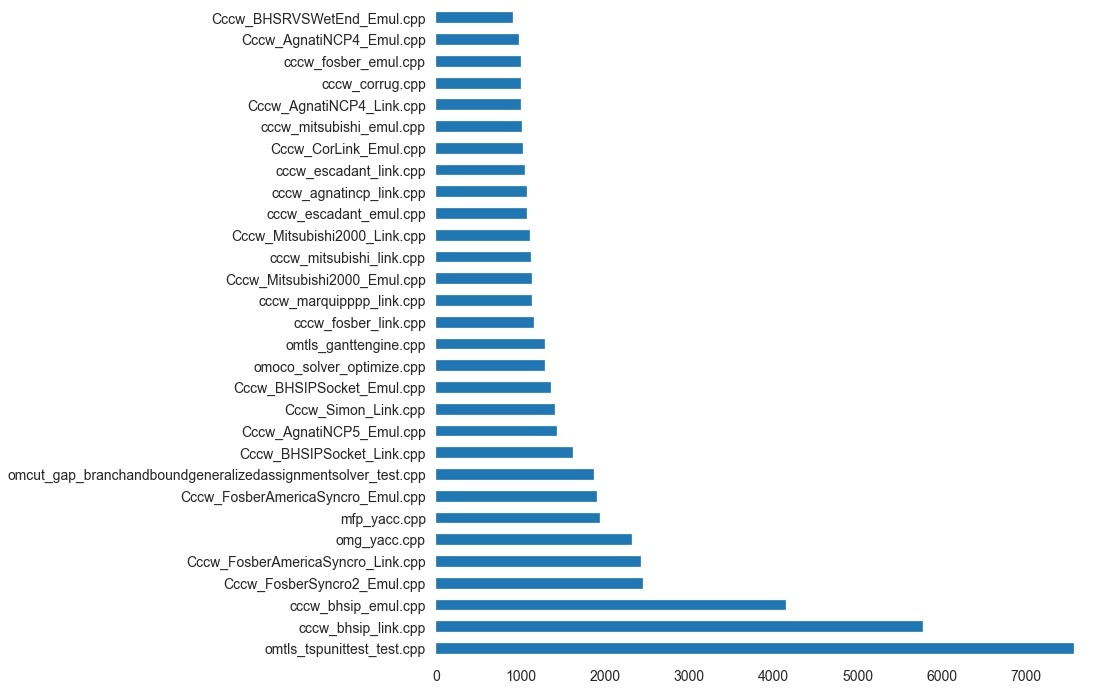
\includegraphics[scale=0.2]{./src/data_analysis/open_file_barh.jpg}
%		\caption{Number of closed alerts in the 30 most represented files}\label{}
%	\end{subfigure}\\
%\end{figure}
%
%
%\begin{figure}[H]
%	\begin{subfigure}{\textwidth}
%		\centering
%		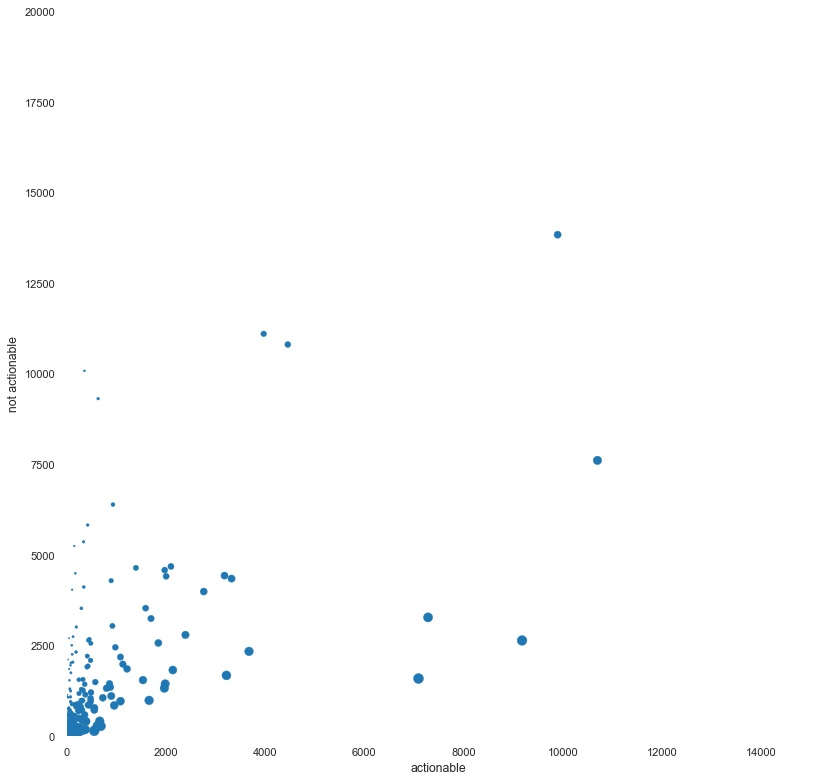
\includegraphics[scale=0.4]{./src/data_analysis/packages_ratio_scatter.jpg}
%		\caption{Scatter plot of open/closed alerts ratio per package (removed some outliers)}\label{}
%	\end{subfigure}\\
%	\begin{subfigure}{\textwidth}
%		\centering
%		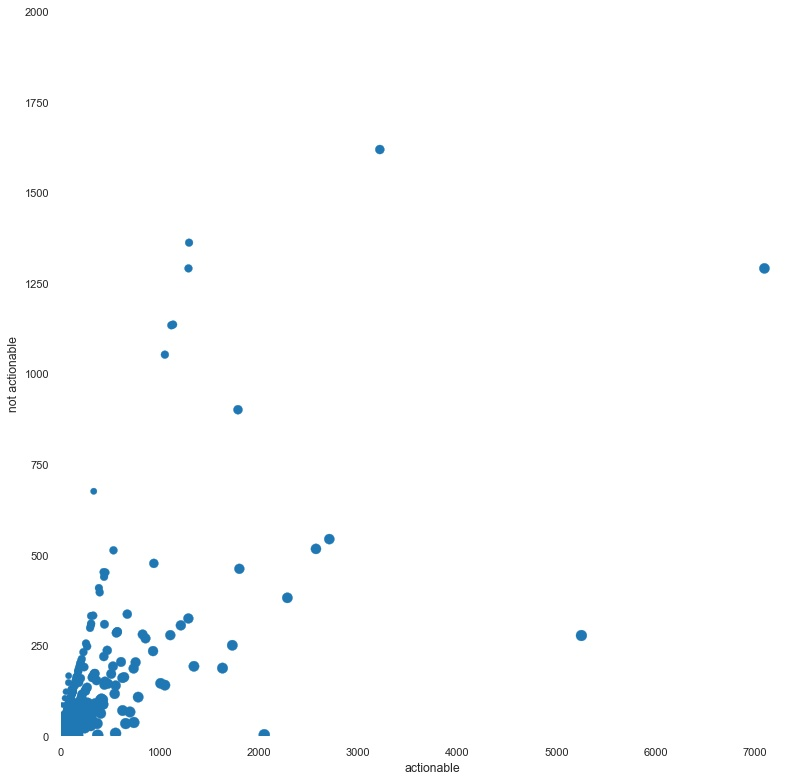
\includegraphics[scale=0.4]{./src/data_analysis/files_ratio_scatter.jpg}
%		\caption{Scatter plot of open/closed alerts ratio per file (removed some outliers)}\label{}
%	\end{subfigure}%
%\end{figure}
%


\subsection{Dealing with unbalanced and noisy data}

Our automatically collected data suffers from two main problems, imbalance and noise. 

Kim et al. \cite{noise_defect} propose a method for dealing with noisy data in the context of defect prediction algorithms. They also provide guidelines for acceptable noise levels and study the impact of different amounts of noise on the prediction performance.
They found out that performance, in terms of f-measure, is affected more by the presence of false positives and that the tested algorithms were robust to the presence of false negatives. When noise levels reach 20-35\% of both FP and FN, the performance decreases significantly, especially on small datasets.
The proposed algorithm for cleaning noisy data by \cite{noise_defect}, calculates the ratio of the top \textit{N} most similar instances of each item that have a different class label. If that ratio exceeds a certain threshold, then that item is considered as noisy.

Batista et al. \cite{balancing_comparison}, perform a comparative evaluation of different dataset balancing techniques. They claim that imbalance alone is not the only reason for poor classifier results, but that it is also related to noisy/overlapping data. According to their experiments, over-sampling methods perform generally better and \textit{SMOTE} + Tomek/ENN provide good results for datasets with few positive examples.

Given the nature of our approach to detecting actionable alerts, it seems plausible that the amount of false positives will be non negligible, and thus there is a high risk that there will be a significant performance impact. Since, the number of examples of the positive class is also smaller than the negative one, there seems to be a necessity to apply a combination of balancing and cleaning to the dataset.

The \textit{imblearn} library (\cite{imblearn}) contains different techniques to clean the dataset by performing under-sampling:

\begin{itemize}
	\item \textbf{Tomek's Links} between two samples is defined as: $d(x,y) < d(x,z) \, and \, d(x,y) < d(y,z)$\\for all other samples \textit{z}. According to the strategy one or both samples forming a Tomek link are removed.
	\item \textbf{Clean dataset by using nearest neighbours}
	\begin{itemize}
		\item \textit{Edited Nearest Neighbours}: applies a nearest-neighbors algorithm and removes samples which do not agree enough with their neighborhood.
		\item \textit{Repeated Edited Nearest Neighbours}: same as before but the algorithm is repeated multiple times.
		\item \textit{AllKNN}: same as before but with each run the number of nearest neighbors is increased.
		\item \textit{Condensed Nearest Neighbors}: uses a 1 nearest neighbor rule to iteratively decide if a sample should be removed (adding a sample at a time to the minority set).
		\item \textit{One Sided Selection}: combines Tomek's Links with Condensed Nearest Neighbors
		\item \textit{Neighbourhood Cleaning Rule} will focus on cleaning the data than condensing them.
	\end{itemize}
\end{itemize}

To see the effect of these methods, we run them on a test dataset. We avoid the two most invasive alerts that together count for more than half of the total number of alerts (around 190k alerts remain).

The following table counts the number of samples cleaned by each method (default parameters):

\begin{table}[H]
	\centering
	\begin{tabular}{cc}
		\hline
		& \textbf{Removed samples} \\ \hline
		\textit{Tomek's Links}                      & 1                        \\
		\textit{Edited Nearest Neighbours}          & 34                       \\
		\textit{Repeated Edited Nearest Neighbours} & 38                       \\
		\textit{AllKNN}                             & 37                       \\
		\textit{Condensed Nearest Neighbors}        & 106949                   \\
		\textit{One Sided Selection}                & 204                      \\
		\textit{Neighbourhood Cleaning Rule}        & 95                       \\ \hline
	\end{tabular}
\end{table}

From seven tested methods only one removes a significant amount of samples (56\% less samples respectively). From further inspection it turned out that the method removed almost all samples of the majority class, which is not something that we want. The other methods have barely an effect on the dataset. That could mean that the dataset does not contain a lot of noise.


\textbf{TO DO: maybe insert before and after graph for data cleaning/balancing? Not enough removed samples!} 
